\chapter{Design and Implementation}

\epigraph{\textit{... where in this snippet $W1$ and $W2$ are two matrices that we initialize randomly. We're not using biases because meh.}}{\rightline{{\rm --- Andrej Karpathy}}}

After researching literature on building libraries from scratch, analyzing pet project source-codes \cite{convnetjs, gibianskysource} and dozens of implementations of professional libraries \cite{TF, caffe, torch},
I concluded that the best way to acquire an in-dept understanding of neural networks is to build my own Deep Learning framework.
This way I had a chance to understand why novel solutions in Machine Learning are formed the way they are.
I also gained insight into what main paradigms are popular libraries based on, such as \emph{computational graphs, parallel processing}, 
and what trade-offs can be made between \emph{computational cost} and \emph{memory usage}, between robustness and plasticity.
Most thankfully, by starting from scratch I have faced situations when theoretical formulas had to be translated into exact working code, which was an important challenge for me.

\paragraph{Goals.} My main objectives when writing code was the following:
\begin{itemize}
    \item[] to make such a library that is able to be extended further
    \item[] open-source, so it can be forked by anyone interested in developing it
    \item[] to make it modular therefore make its usage independent of the task
    \item[] use the fewest possible technical tricks for sake of simplicity
    \item[] to stay as close to pure mathematical formulation of the classical paradigms as possible
    \item[] put emphasis on ease of use and understanding
\end{itemize}
\paragraph{Disclaimer.} Apart from \textbf{NumPy} and its complementary package \textbf{SciPy}, no external libraries and dependencies are used in the implementation. 
I want to emphasize that this work was not written to compete with contemporary state-of-the-art frameworks, rather to help perceive the general ideas behind novel researches, and to encourage interested fellows to carry out researches on their own.
\clearpage
\section{Choice of design pattern and language}

The formulas of classical neural networks, whose nodes are organized into
 lattices forming a Directed Acyclic Graph, shows minor variance in
 contents of independent sources. Still their common point that they rely
 on basic vector algebra and functional analysis, therefore considering
 arrays representing general mapping functions, as their core building
 blocks is a paradigm which would not interfere with the current formal
 and informal descriptions of deep learning.

\subsection{Disassembling a universal approximator}
Thinking of a neural net as a function \(\mathcal{F}\), is implicitly a black-box representation of the paradigm.
Users of different applications which offer feature detection, segmentation, prediction, etc. are using this function without knowing what exactly happens behind the curtains. 
Further investigating $\mathcal{F}$, we can constrain it to have a DA computational graph, also to have the nodes of the graph arranged to lattices.
Practically it means that the perceptrons making up the layer \(l\) are strictly projecting $F_l$ their \textbf{inputs} 
$ x_l \in \mathbb{R}^N $ \emph{forward} to scalars, which if all perceptrons are evaluated in parallel, forms the 
\textbf{output} $y_l \in \mathbb{R}^M$, have no feedbacks and loops. 
This projection of layer $l$ can be written as $y_l = F_l(x_l)$. 
Intuitively the input of the next $(l+1)^{th}$ layer will be the output of the previous layer:
$x_{(l+1)} = y_l$.
For the sake of simplicity I excluded Recurrent Networks from the space of $\mathcal{F}$, but later the definition can be extended for vanilla recurrent networks and LSTM networks as well.

\subsection{Language} Keeping in mind that using a general high-level language (like MATLAB) can yield poor computational efficiency, making benchmarks, testing and applications ponderous.
Also considering a low-level language (like C) 
would distract us from the main goal, all 
the time is spent on optimizing further and 
further the basic algorithms, and usage usually 
results in boilerplate codes. 
Either way it would make the implementation unclear for those, who did not participate in the designing of the library.
I wanted to chose a language which offers an optimal solution for this challenge, is flexible, well documented and simple enough for newbies to catch up.
Because of the support of both object-oriented and procedural approaches and offering the above, I choose Python.

\subsection{Design pattern} While designing blueprints of the implementation, I examined the Neural Networks as universal approximators in a \textsc{top-down} manner.
I have disassembled them to basic blocks, abstracting the function of each level.
Later I used these units in \textsc{bottom-up} approach to create an object-oriented hierarchic model that realizes simple operations and is well defined on every level: granting a universal interface to be further extended.


\section{Single Layered networks}
For example if a small picture is given to a person, he or she guesses about it. If that person is told that there are four classes, 
like \emph{Car, Plane, Cat, Kid}, he can tell how likely it is that 
the given picture falls in that class, so he can give a so-called \emph{confidence parameter}.
Patterns which are associated with cats may be associated with kids too, but is unlikely to be associated with planes. Deciding whether a pattern improves the confidence on each class or not, yields a \textbf{sign} for the given pattern, and the measure how strongly it influences the likelihood is called the \textbf{weight} of the pattern.
In \emph{neural networks} there are small nodes based on the biological model of neurons, that is responsible for recognizing and weighting the patterns. These nodes are called \textbf{perceptrons}. 

\subsection{Defining the Perceptron} 
Let be $x$ a preprocessed information, the perceptron $\mathbf{P}$ decides which parts of it are important in recognizing a cat: having a corresponding weight with large magnitude, and which of them are irrelevant: having a weight with magnitude close to zero. 
Therefore a \emph{perceptron} has a weight $w_i$ for each input $x_i$ and its transient state can be now formally written:
$$
	\mathbf{P}_{transient}=\sum_i x_i w_i
$$
Which can be also rewritten as the inner product of $\mathbf{x}$ and $\mathbf{w}$

$$
	\mathbf{P}_{transient}= <\mathbf{x} \;,\; \mathbf{w}>=\mathbf{x}^T\mathbf{w}
$$
In the following examples perceptrons will be arranged in a special way, to form a \textbf{Feed Forward} network, meaning that the information flow will occur in a direct way, without feedbacks, see figure \ref{fig:ff}.
However wiring many perceptrons together results in a numerically unstable system, caused by the lack of any restriction on the magnitude of the weights.
Regularization addresses exactly this problem, implicitly making the network less likely to simply memorize pictures, or only respond to samples from the training set -- the problem of overfitting.

\begin{figure}
	\centering
	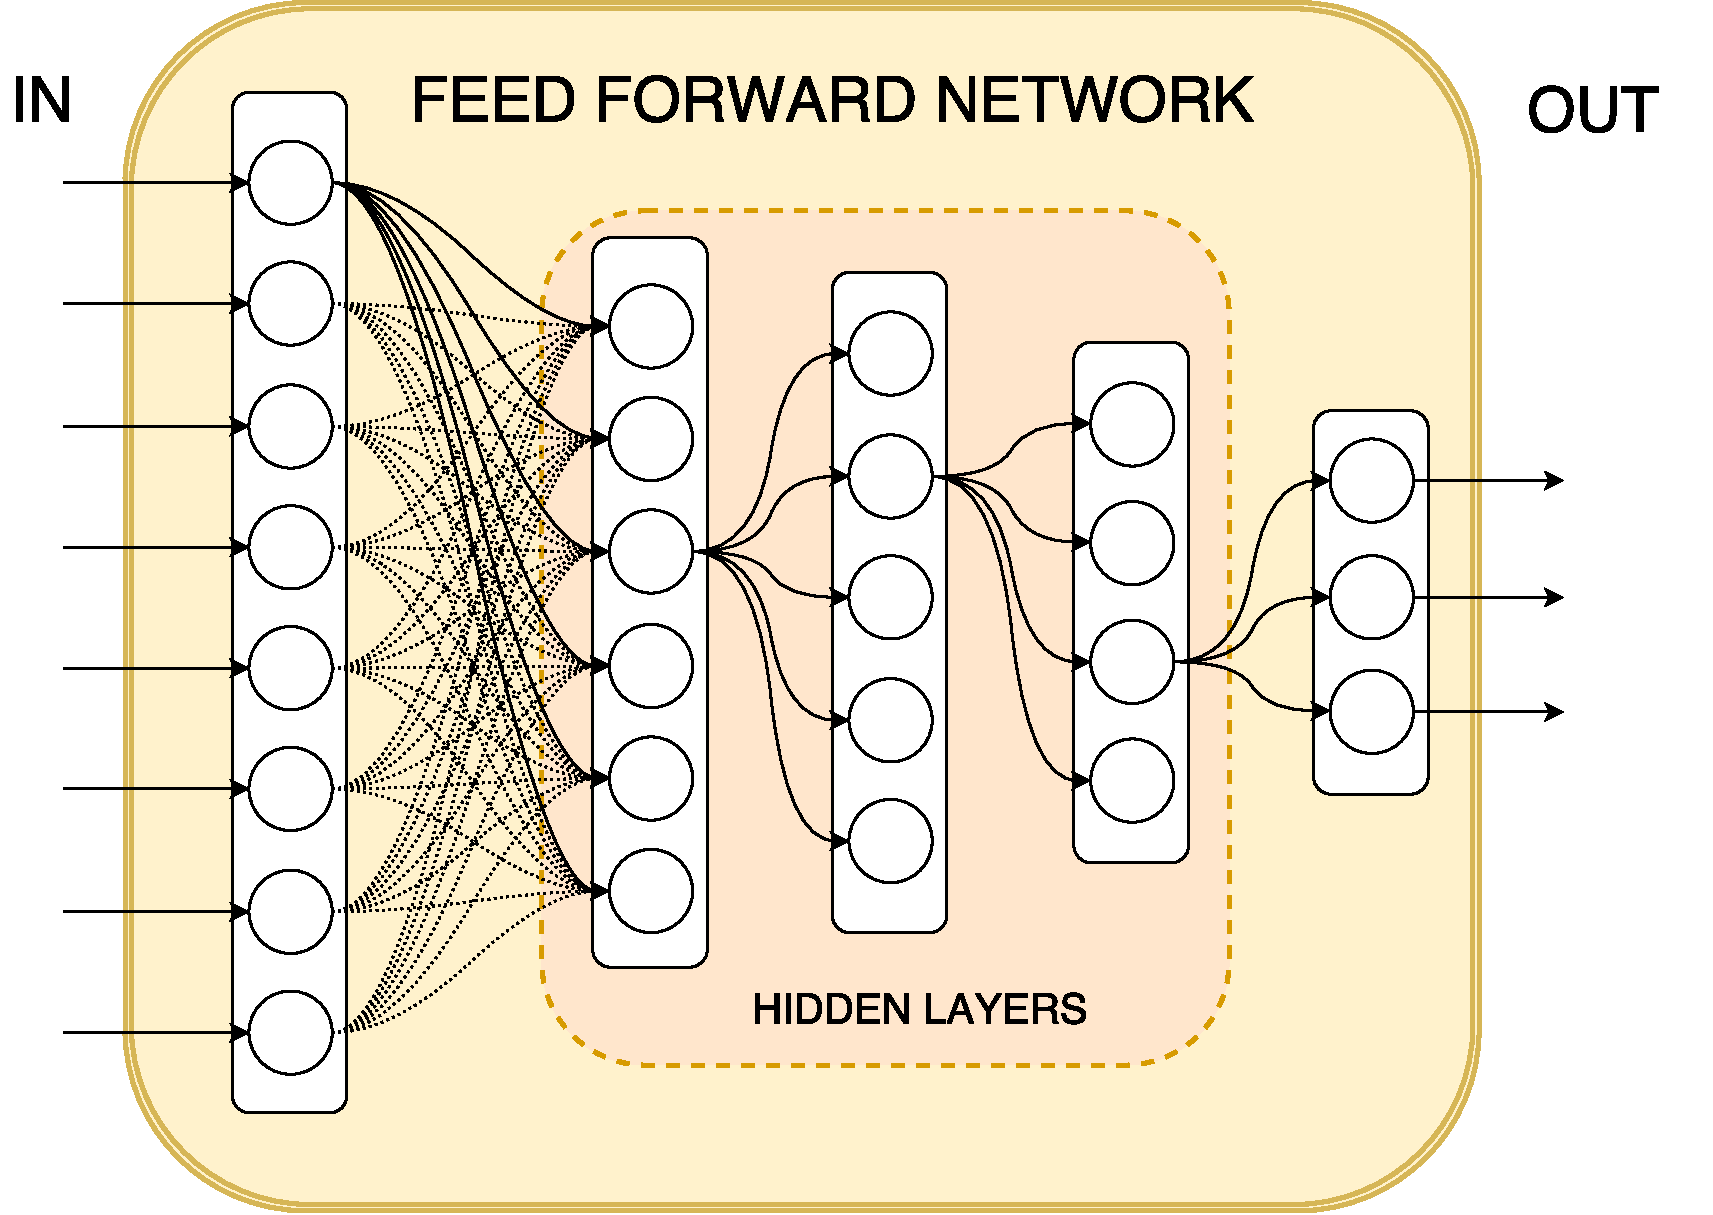
\includegraphics[width=0.6\textwidth]{smallnetwork.pdf}
	\caption{A small feed forward network with three hidden layer composed of Fully Connected layers.
	}
	\label{fig:ff}
\end{figure}

\subsection{Basics of Learning}
After describing the model, the first question is:
\begin{flushright}
    \emph{--- what are the correct values for $\mathbf{w_P}$ for each $   
    \mathbf{P}$ in network $N$?} \\ 
\end{flushright}
There are a lot of intuitive explanations how this problem should be approached and solved. For exhaustive investigation of the topic, visit Michael Nielsen's website \cite{nnsdl}. 
Anyhow, in general this is still the most studied question in machine learning. 
Luckily, if $N$'s performance can be measured, thanks to its feed-forward structure a \emph{numerical suggestion} can be defined as well, which tells how to change $\mathbf{w_P}$ to improve efficiency of $N$. In practice an $\mathbf{E}$ error function is defined, and the objective of the training is to reduce it. Without digging deep in math we can find an intuitive situation with the same results.\\

Take a perceptron $\mathbf{P}$ with input $\mathbf{x}$ of objects on a given picture of a cat. Suppose that this perceptron \emph{fires} (has high output value) when wheels are on the picture. It should remain silent when there are no round objects listed in 
$\mathbf{x}$, still it turns on, affecting the output of $N$, producing high error.
Since we know the original label of the picture, we can tell which assumptions were wrong, and which were good - which to decrease, which to increase if the next time $N$ is given the same input. 
This information is distributed between the previous perceptrons which caused the current one to fail, by simply multiplying the error with the weight corresponding to the previous node. 
Also with the information of how much the output of the actual node influenced the error, and with its input values, the significance of misleading $\mathbf{x_i}$ can be reduced, and important features' weights can be increased, which is actually finding a better $\mathbf{w_P}$.
For further intuitive examples see section \ref{sec:diff}, or visit Andrej Karpathy's guide \cite{karpathyblog}.

\paragraph{SGD.} The example concluded to the practical application of the so called \emph{Stochastic Gradient Descent}. 
Originally every samples in the training set should be introduced to the system before updating its weights and that would be the \emph{Gradient Descent}, but in  the hope that the samples falls in a subset of the whole space of all possible inputs, the algorithm uses mini-batches for the learning process. When the number of samples in the batches reduces to 1, the training is called on-line training. And if it happens on $N$ containing a single perceptron it is called \emph{Rosenblatt perceptron learning algorithm}.


\section{Inference}
Let us suppose that for a particular task an $\mathcal{F}$ is given, first what we have to understand is how input data 
$x \in \mathbb{X}$ (interchangeably $x_1$) is inferred.
First, assume that the data can be expressed as multi-dimensional matrix, like RGB pictures, audio recordings, gene maps.
Some networks preserve the spatial information i.e. feature extraction performed on images, 
while other instances operate on the whole input data i.e. processing audio samples in frequency domain.
Either way the output $y$ (or $y_L$) can be obtained by feeding $x$ to the network: 
$ y = \mathcal{F}(x)$
The core concept is that we can compose such an $\mathcal{F}$ function by applying multiple projections to $x$.
Practically that means sending input through the first layer, the second, and all the way through to the last layer $L^{th}$, which output would be the value of $\mathcal{F}(x)$, the response of the network.
Therefore in terms of evaluating $\mathcal{F}(x)$ layer by layer, actually translates to a single function call, which can be unfolded to a sequence of embedded projections:
$$
    \mathcal{F}(x) = F_L \left( x_L \right) = F_L \left( y_{(L-1)} \right)
$$
$$
    F_L \left( y_{(L-1)} \right) = 
    F_L \left( F_{(L-1)} \left( x_{(L-1)} \right) \right) = F_L \left( F_{(L-1)}\left( \cdots F_1(x)\right)\right)
$$
Using the function composition operator $\circ$, rewritten in the classical notation:
\begin{equation}\label{eq:forward}
\begin{split}
    \mathcal{F}(x) = F_L \circ F_{(L-1)} \circ \cdots \circ F_1(x)
\end{split}
\end{equation}

The \ref{eq:forward} equation is the most fundamental idea behind feed-forward neural networks, namely the \emph{inference} or \emph{forward-propagation}
As mentioned above, every layer $l$ is represented by an $F_l$. 
The most basic layers are the \emph{Fully Connected} and \emph{Activation} layers.

\subsection{Fully Connected layer} 
These layers carry out the heavy-lifting of inference by performing linear projection and translation transformations. 
The operations are following the rules of basic linear algebra, where the input $x_{FC} \in \mathbb{R}^N$ and the output $y_{FC} \in \mathbb{R}^M$ are specified as real valued vectors.
The parameters of the layer $\phi_{FC}=(W, b)$ are the corresponding weights and biases of each perceptron node in the layer forming a \emph{weight matrix} $W \in \mathbb{R}^{M \times N}$ and a \emph{bias vector} $b \in \mathbb{R}^M$ respectively.
Therefore evaluating the output of the Fully Connected layer is the defined by the following:
\begin{equation}\label{eq:FC}
\begin{split}
    y_i &= \left(\sum_j  W_{i,j} \; x_j \right) + b_i \\
    y &= W \cdot x_j + b \\
    \left[M\right] &= \left[M \times N\right] \cdot \left[N\right] + \left[M\right]
\end{split}
\end{equation}

\subsection{Activation layer} 
Nodes in activation layers are introducing non-linearity to the network, 
by applying the same non-linear activation function to the corresponding output of the previous layer, performing element-wise operation.
Let $F$ be an activation layer with activation function $f$ after a fully connected layer with 3 neurons:
\begin{equation*}
    F(x) = \begin{pmatrix}
    f(x_1) \\ 
    f(x_2) \\
    f(x_3)
    \end{pmatrix}
\end{equation*}
These functions are essential for the network, since they increase the numerical stability: they \emph{squeeze} or \emph{mitigate} the input preventing the network from \emph{saturation} or \emph{explosion} (numerical of course). Conventionally the following functions are applied most often as activation function:
\begin{align}
    \mathrm{Rectified Linear Unit (ReLU) := } &max\left\lbrace 0, x \right\rbrace \label{eq:af1} \\
    \mathrm{Hyperbolic Tangent (TanH) := }   &\tanh(x) = \frac{2}{1+e^{-2x}}-1 \label{eq:af2}\\
    \mathrm{SoftPlus (SP) := }   &\ln(1+e^x) \label{eq:af3}\\
    \mathrm{Logistic (Log) := }  &\frac{1}{1+e^{-x}} \label{eq:af4}
\end{align}
The only constraint on these functions that they have to keep the dimension of the input, namely $F_{act}:\mathbb{R}^N \mapsto \mathbb{R}^N$.
\emph{Note:} These functions do not have any variable parameters, therefore activation layers cannot be trained.

\section{Measuring efficiency}
If the function $\mathcal{F}$ mentioned above is given, and satisfies our needs, then we are done.
However this is usually not the case, and finding the optimal $\mathcal{F}^*$ is the main challenge targeted by many branches of Machine Learning.
Despite it was proven, that standard multilayer
feed-forward networks are capable of approximating
any measurable function to any desired degree of
accuracy \cite{hornik1989multilayer},
if the goal function $\mathcal{F}^*$ is unknown, 
or too abstract to be \emph{measurable} (i.e. telling how funny a picture is), 
we cannot utilize the universal approximator.

\subsection{Loss} 
By reformulating the objective, we can define a Loss function $\mathcal{L}:\mathcal{F}(\mathbb{X}) \mapsto \mathbb{R}$,
which maps our candidate $\mathcal{F}$ network to a scalar field, that represents the general correctness of $\mathcal{F}$ over the space of possible inputs $\mathbb{X}$ -- the lower its value the better $\mathcal{F}$ is performing.
By doing so we may apply Machine Learning algorithms that would \emph{minimize} the Loss, therefore $\mathcal{F}$ would converge towards $\mathcal{F}^*$ implicitly.

\emph{Note:} In practical implementations $\mathcal{F}$ is not evaluated over the whole space of possible inputs, instead in the hope that a small subset of both \emph{training} and \emph{validating} samples called a mini-batch will approximate $\mathcal{L}(\mathcal{F})$ as well. Useful practices for reducing computing complexity and improving stability, and rate of convergence will be covered later.


\subsection{Supervised learning}
In cases where the parameters of $\mathcal{F}^*$ are not known,
but we know how it would map the input space $\mathbb{X} \mapsto
\mathbb{Y}$, e.g. which character appears on the input image $x$, 
then we  can define a set of previously \emph{labeled} pairs of input - 
solution sample which could be used later on for training, and
evaluating performance of the network.

\subsection{Unsupervised learning}
When no labeled dataset is available, the network still can be used for extraction of hidden structure of the unlabeled samples. Later these instances are used as density estimators, or adapted as feature extractors for larger networks.
\textbf{Generative Networks.} Training such architectures can be done by feeding networks random noise as input and training them to reproduce given samples: $\mathcal{F}:\mathbb{R}^k \mapsto \mathbb{X}$, hence the name \emph{Generative Networks}.

\textbf{Auto-encoder Networks} The other frequently applied paradigm is setting the objective task to compress the input sample into a $h \in \mathbb{R}^k$ hidden representation vector that is able to preserve the key information about the original input, and either by symmetric (Restrictive Boltzmann Machines) or independent (Deep Belief networks) operations decompress the data.

In both cases hyper-parameter $k$ is intuitively the number of unlabeled features in the \emph{latent space} that the network will be able to categorize, i.e. correlation between different color intensities on pictures taken of stained brain samples.


\section{Adjusting parameters}
Generally speaking, applying Machine Learning algorithms boils down to the process of iteratively altering parameters $\phi$ of $\mathcal{F}$ to optimize the Loss.
Once $\mathcal{L}(\mathcal{F})$ is obtained, we can evaluate how changing the parameters would influence it -- evaluate the gradient $\nabla_\phi \mathcal{F}$ of the parameters  with regards to $\mathcal{L}$.

\subsection{Gradient Descent}
Updating $\phi$ by descending on the gradient slope with a small step size $\epsilon$ will decrease $\mathcal{L}$.
Derivation from the general form of Gradient Descent depends on the architecture of the network, 
but there is a main concept for doing so, called Backpropagation described by Werbos \emph{et al.} \cite{werbos1994roots}. 
The exact method which can be applied for Fully Connected networks 
will be explained in detail in section \ref{sec:diff}.

\subsection{Training Policies}
Though theoretically after finite steps of iterations, with Gradient Descent $\mathcal{F}$ may approximate any Borel-measurable function, 
in practice Deep Neural Networks can fall into local-minimum of the parameter-space.
I.e. the network tends to learn the very basic features of the input space, if it is not forced to generalize.
The problem with generalization is that the training set has finite samples and extending it requires human-supervision.
Therefore training networks with many layers requires some advanced techniques for training.
There are multiple way to improve the \emph{convergence rate} and the \emph{stability} of the network.

\paragraph{Batch processing.} There are two radical methods of updating the parameters in the network. 

Theoretically if we wanted to create a perfect network, we would infer all possible samples from $\mathbb{X}$ and the Loss function 
$\mathcal{L}$ would evaluate the network on every solution (in a single iteration, without the network being updated), 
then we would take the mean of the Loss to evaluate the gradient, e.g. 
$$\mathcal{L}^*=\frac{1}{N}\sum_{x \in \mathbb{X}}\mathcal{L}(\mathcal{F}(x))$$
This way, if the capacity of $\mathcal{F}$ is large enough, it is possible to train the network to be able to solve every problem.
In a special case when we want to simulate logical circuits with real values instead of Boolean \texttt{true} or \texttt{false},
then we can train a network to act like a logical processing unit - since we are able to map $\forall x \in \mathbb{X} \mapsto y \in \mathbb{Y}$ by 
external evaluation.

The other case is more practical, when the network is updated \textbf{on-line}, described exhaustively in \cite{onlinelearn}. 
In a nutshell on-line training is when the network after initialization, is utilized as well.
Predictions which were correct are put into the training set, and the network weights are updated immediately 
to encourage the same response for similar samples.
A frequent application of on-line training is called \emph{Q-learn}, for case studies see \cite{qlearn-case}.

Both methods are powerful for specific tasks, but in practice taking the golden mean is considerable:
Inferring multiple samples at the same time with the same network not just yields a more stable convergence, 
but is an excellent opportunity to parallelize the process:
Extending by one extra dimension to each stage of the inference (inputs, transient activations, outputs) can be done easily,
also almost every library can take the advantage to perform optimized matrix operations on multidimensional matrices (at least \emph{NumPy} can).
On the second hand, processing only \emph{some} instead of all of the input samples at once is computationally a better choice.
In real applications it is worth considering $2^k$ mini-batch sizes because of the memory allocation \cite{stanfordlectures}.

\paragraph{Advanced First order derivatives.} 
Simple heuristics applied to first order derivatives, such as:



\begin{description}[align=right,labelwidth=3cm]
\item[Momentum] \cite{sutskever2013importance}
    $v_{(n+1)}=\gamma v_{n} + \nabla_{\phi_n}\mathcal{L}$ and 
    $\phi_{(n+1)} = \phi_n -\epsilon v_n$
\item[Adagrad] \cite{duchi2011adaptive}
    $r_{(n+1)}=r_n+\left(\nabla_{\phi_n}\mathcal{L}\right)^2$  and 
    $\phi_{(n+1)} = \phi_n - \frac{\epsilon}{\gamma + \sqrt{r_n}} \left(\nabla_{\phi_n}\mathcal{L}\right)^2$ (element-wise) 
\item[RMSProp] \cite{rmsprop} $r_{(n+1)}=(1-\epsilon)r_n + \epsilon\left(\nabla_{\phi_n}\mathcal{L}\right)^2$
\item[Adam] \cite{kingma2014adam} Combination of RMSProp and momentum.
\end{description}
A more sophisticated, but expensive method is using second order derivative, for instance Conjugate gradient \cite{shewchuk1994introduction}.

\paragraph{Decreasing the learning rate $\epsilon$.}
For large networks it is inevitable to use decreasing learning rate, otherwise the convergence would take too much time (small $\epsilon$) or would not even occur (large $\epsilon$). 

\paragraph{Cross-Validation.} Special $\hat{\mathcal{L}}=(\mathcal{L}_{train}, \mathcal{L}_{validation})$ functions approximate the efficiency of the network not just by evaluating them on the currently or previously trained samples, but on samples which are from a totally \textbf{disjunct set} $\mathbb{X}_{validation}$.
The motivation behind it is to see how well would the network perform on samples which it have not faced before.
By doing so we can evaluate how well the network \emph{generalized} the information from samples of the training set.
In order to keep $\mathbb{X}_{train} \bigcap \mathbb{X}_{validation} = \varnothing$ we may not use $\mathcal{L}_{validation}$ for parameter updating.
However in order to \textbf{prevent overfitting} we can monitor e.g. generalization error $E_g=\frac{\hat{\mathcal{L}}_1}{\hat{\mathcal{L}}_2}$ during training 
and use \textbf{Early Stopping} when $E_g > \delta$, where $\delta$ is a parameter of how much we tolerate overfitting.

\subsection{Networks in practice} 
Though networks can vary in shape and function, the representation of the succeeding layers, evaluated by embedded functions described in \ref{eq:forward} is a common feature. Each of these layers serve as nodes of the computational graph of the network. The type of the layer determines whether it can be updated or not: for \emph{Fully Connected} layers $\nabla_\phi F_{FC}$ is well defined, explained in the following example.

\paragraph{Toy example.} 
Assume $\mathcal{L}$ is given, and we have a fully connected network with 2 hidden layers, i.e. $L=3$, which maps a $N$ dimensional input vector $x$ to a $M$ dimensional output vector $y$, namely $\mathcal{F}:\mathbb{R}^N \mapsto \mathbb{R}^M$. The constraint on the parameters are:
\begin{itemize}
    \item[] $W^1$ of the first layer must have $N$ columns
    \item[] $W^3$ and the bias $b^3$ of the last layer must have $M$ rows, dimensions respectively.
    \item[] Number of rows of $W^l$ must match $dim(b^l)$ $3$ dimensional
    \item[] Number of columns of $W^l$ must match $dim(b^{(l-1)})$
\end{itemize} 
Then the evaluation unfolded would look like the following: 
$$y = \mathcal{F}(x) = F_3 \circ F_2 \circ F_1(x) = W^3(W^2(W^1(x)+b^1)+b^2)+b^3$$
For further usage and simplicity, I would like to fix these numbers.
Let $\mathcal{F}$ be a network with the following \emph{shape}: $\left[5, 4, 3\right] $
meaning that in each layer there are 5, 4, 3 neurons respectively, $M=3$ and all nodes are connected to the previous layer. The width of the input layer is not yet defined, let it be $N=10$. 
\emph{Note:} It is usually distracting and redundant to explicitly write the width of the outermost layers when testing different networks, because the input and the output layers must have fixed dimension for the same task, while the width of the hidden layers are varied.
Define an $L_2$ Loss function on the toy example. For one sample-label pair $(x,y^*)$ the $L_2$ Loss is:
\begin{equation}
    \mathcal{L}_2(\mathcal{F}) = \frac{1}{2} \sum_{i} (y_i^* - \mathcal{F}(x)_i)^2 = \frac{1}{2} \sum_{i} (y_i^* - y_i)^2
\end{equation}
$L_2$ is a universal Loss function, which is used in cases where the label space $\mathbb{Y}$ is continuous (e.g. floorspace, consumption and height of a house, based on the price: $\mathbb{R}^1 \mapsto \mathbb{R}^3$).

\section{Differentiation}\label{sec:diff}
In the above evaluating of $\nabla_\phi \mathcal{F}$ can be done in two ways, namely by numerical approximation, or by analytical derivation, in the following I will discuss both.

\subsection{Numeric differentiation} Evaluating the numerical gradient (or difference) is an elementary, yet powerful operation, in which we would \emph{perturb}, or modify one parameter $\phi$ of our system $\mathcal{F}$ at once.
That is done by first adding $\phi^+$ and after subtracting $\phi^-$ a little amount $d\phi$ from the original $\phi$ and evaluate $\mathcal{L}^{\pm}=\mathcal{L}(\mathcal{F}_{\phi^{\pm}})$, namely the \emph{Loss} of the system in the modified state, yielding the numerical gradient in the following equation:

\begin{equation} \label{eq:numgrad}
    \frac{d\mathcal{L}(\mathcal{F})}{d\phi} = 
    \frac{\mathcal{L}^+ - \mathcal{L}^-}{2 d\phi} = 
    \frac{\mathcal{L}(\mathcal{F}_{\phi^+}) - \mathcal{L}(\mathcal{F}_{\phi^-})}{2 d\phi}
\end{equation}

\paragraph{Summary.} In a nutshell value of $\frac{d\mathcal{L}(\mathcal{F})}{d\phi}$ tells how changing the parameter $\phi$ by $d\phi$ would change the performance of the network. If it is positive then updating $\mathcal{F}$ by adding $d\phi$ to $\phi$ would result in higher Loss value, which is the opposite of our goal, so we just subtract it, if it is negative, then trivially we should add $d\phi$ to $\phi$ since it is making some good progress.

\subsection{Complexity} 
Though letting the computer do the hard work seems to be a good idea, it is worth considering that the simple method above will be applied to every $\phi$ of $\mathcal{L}$.
It means that for the network in the toy example, we need to evaluate $\mathcal{L}(\mathcal{F})$ two times for each parameter in 
the weight matrices and the bias vectors of the network, totaling in 
$$\#(\phi) = 2\times\sum_{i=1}^3 N_{(i-1)}\cdot N_i + N_i = 2\times(10\cdot 5 + 5 ... + 4\cdot 3 + 3) = 188$$
Even if $\mathcal{F}$ is approximated by using $k$-sized mini-batches for evaluation it is still a computationally very expensive function, because the inference would result in the following number of operations of addition and multiplication:
$$\#(\mathrm{operations}) = k\times\sum_{i=1}^3 2\cdot N_{(i-1)}\cdot N_i + N_i = k \times 176$$
Therefore approximated with $k=10$ mini-batches would a single parameter update of a very tiny network would require total operations of:
\begin{equation}
    \#(\mathrm{total})=\#(\phi) \times k \times \#(\mathrm{operations}) = 188 \cdot 10 \cdot 176  = 330880
\end{equation}
Because both $\#(\phi)$ and $\#(\mathrm{operations})$ has complexity of $\mathcal{O}(N^2)$, one update will yield complexity of 
\begin{equation}
    \#(\mathrm{total})=\mathcal{O}(N^4)
\end{equation}
We can see that even for a shallow and relatively small network (industrial AI networks has billions of parameters, and uses much larger batches) described in the toy example the method is really costly.
That encourages us to derive our differentials on paper first, and use \emph{numerical gradient approximation} for checking our solution. Using \emph{Gradient Check} is essential when implementing new architectures, because it is a very efficient tool for debugging in comparison with updating. The method in a few words is about setting an error rate $\epsilon$, and decrease $d\phi$ until the numeric solution does not match the analytic solution with $1-\epsilon$ significance. If the analytic solution is incorrect the cycle will not terminate.

\subsection{Analytic differentiation}
Deriving the update by hand requires basic knowledge in calculus extended to multivariate cases, though since the operations are elementary, in general we must understand only three basic definitions to do so. 
Some formality before starting: we have three independent variables $x$, $y$, $z$ and functions $f$, $g$, $h$. The result of operations performed on variables, i.e. $x+2y$ can be represented by a function $f=x+2y$. 
If the value depends on a variable then it can be written explicitly, passing the variable as \emph{the argument} of the function $f(x,y)=x+2y$. 
For the sake of simplicity assume that the variables are not general objects from an abstract space, they are only real values: $x,y,z\in \mathbb{R}$. However the following description could be extended for the above-mentioned variables as well. For any one-dimensional function $f(x):\mathbb{R}\mapsto\mathbb{R}$ we say that the value represented by the function depends on the variable by the extent of its derivative. The derivative (or differential) of the function can be seen as an ideal case of \ref{eq:numgrad} where the perturbation would approach zero, namely:
\begin{equation}
    \frac{\partial f}{\partial x} = \lim_{dx\rightarrow 0}\frac{df(x)}{dx}= \lim_{dx\rightarrow 0} \frac{f(x+dx)-f(x-dx)}{2dx}
\end{equation}
\paragraph{Multiplication rule.}
Consider a value $x\cdot y \cdot z$ represented by $f(x,y,z)$. $f$ is now depending on three variables, we can define the measure of this dependency on one variable by the formal equation:
\begin{equation*}
\begin{split}
    \frac{\partial f}{\partial x} = \lim_{dx\rightarrow 0} \frac{f(x+dx,y,z)-f(x-dx,y,z)}{dx}
    &= \lim_{dx\rightarrow 0} \frac{((x+dx)\cdot y \cdot z)-((x-dx)\cdot y \cdot z)}{2dx} \\
    = \lim_{dx\rightarrow 0} \frac{(x+dx)-(x-dx)}{2dx} y z&= \lim_{dx\rightarrow 0} \frac{2dx}{2dx} yz= yz
\end{split}
\end{equation*}
We can apply the same method for each variable, the result will be the elements of the \emph{gradient} $\nabla f$
\begin{equation}\label{eq:multiplication}
    \frac{\partial f}{\partial x} = y z \qquad
    \frac{\partial f}{\partial y} = x z \qquad
    \frac{\partial f}{\partial z} = x y 
\end{equation} 
The important thing to understand that in a computational graph, a multiplicative node, which takes $N$ arbitrary parameters (or arguments), will have a \emph{partial derivative} for each variable its output is depending on. In general if these derivatives are represented as a vector, then it is called the gradient $\nabla f$ of $f$. Also the value of the derivative will be the product of all variables except the one of which we are computing the influence of on the output.

\paragraph{Addition rule.}
Consider a value $x\cdot y + x\cdot z$ represented by $g(x,y,z)$.
The change of $g$ with respect to $x$ is defined with the following shortened equation:
\begin{equation}\label{eq:addition}
    \frac{\partial g}{\partial x} = \lim_{dx\rightarrow 0} \frac{((x+dx)y +(x+dx)z)-((x-dx)y +(x-dx)z)}{dx}=y+z
\end{equation}
Notice that -- in the terms of computational graphs -- if a node contributes to other different operations (namely $x\cdot y$ and $x\cdot z$), 
than the derivative of each occurrence in \emph{later} values will be summed up. 

\paragraph{Chain rule.}
Let $f(x)=2x+3$ and $g(f)=5f$. Suppose that we would like to know the derivative of $g$ with respect to $x$.
At first we cannot do so, but there are two options: in the hope that substituting the value represented by $f$ into $g$ would not make the equation too complex we can unroll the references and rewrite $g(x)=5\cdot(2x + 3)$, or we could use the chain rule:
$$
    \frac{\partial g}{\partial x} = \lim_{dx \rightarrow 0} \frac{g(f(x+dx)) - g(f(x-dx))}{2dx}
$$

\begin{center}
    Assume that $f(x+dx)-f(x-dx) \neq 0$.
\end{center}

$$
    \lim_{dx \rightarrow 0} \frac{g(f(x+dx)) - g(f(x-dx) ) }{f(x+dx)-f(x-dx)} \cdot \frac{f(x+dx)-f(x-dx)}{2dx}
$$

\begin{equation}\label{eq:chain}
    \frac{\partial g}{\partial x} = \frac{\partial g}{\partial f} \cdot \frac{\partial f}{\partial x}
\end{equation}

Which is a formula of the products of partial derivative of $g$, that treats $f$ like a variable, and $f$ explicitly operating on variable $x$.
The derivative of $g$ with respect to variable $x$ is the product of the \emph{local derivative} of $g$ is $\frac{\partial g}{\partial f}=5$ and $\frac{\partial f}{\partial x}=2$ which equals $\frac{\partial g(x)}{\partial x}=\frac{\partial(5\cdot (2x + 3))}{\partial x} = 10$, the function strictly depending on $x$.
The important message is that we can interchangeably use function values and variables with a constraint that at a point, in an arbitrary depth there must be a real variable.
\emph{Note:} the statement above stands for computations with \emph{Acyclic Graph}, meaning that there should not be any feedbacks or loops -- no definitions like $f(g), g(f)$ or $f(f)$.
We will see that these rules play a very fundamental role in training networks.

\paragraph{Vector Notation.}
Before drilling deep into mathematical equations, a small reminder: the following vector and matrix formulation is just a special annotation, 
using the rules above, which helps to make clear both the definition, and the computations done by the network when it is implemented. 
The vectors with partially derivatives inside are just representing \emph{real values}, arranged in a fancy way.
Every vector and matrix defined in forward propagation, has its corresponding derivative w.r.t. the Loss.
More trivially, if any value is depending on a list of variables $f(x_1, x_2 \cdots x_n) = f(\mathbf{x})$ (a vector) then there is a list of \emph{partial derivatives} w.r.t. to $f$ -- forming the gradient $\nabla f = \left(\frac{\partial f}{x_1}, \frac{\partial f}{x_1} \cdots \frac{\partial f}{x_N}\right)$. 
\emph{Notation}: When the vector notation is emphasized the variable name is conventionally written in bold font $\mathbf{x}$, or is underlined \underline{$x$}.
Because later the indexing would become too crowded, we only use the indexed notation when it is necessary, otherwise using $x$.

The next step is formulating the dependency of multiple functions on multiple variables.
As seen above, a multivariate function has its gradient vector --
in the same fashion as the list of variables were organized into vectors $\mathbf{x}$, values composed of them can also form a vector $F = (f_1, f_2 \cdots f_M)$, composing a multivalued function depending on the same variables.
Doing so yields a first-order derivative matrix, composed of gradient vectors $J=(\nabla f_1, \nabla f_2 \cdots \nabla f_M)^T$, called the \emph{Jacobian of $F$}.
The Jacobian has as many rows as output values $F$ has, and the same number of columns of the variables that $f_i$ is a function of.
\begin{equation}\label{eq:jacobian}
    J(F) = 
    \begin{pmatrix}
    \quad \nabla f_1 \quad \\ 
    \vdots \\ 
    \nabla f_M
    \end{pmatrix} 
    =
    \begin{pmatrix}
    \frac{\partial f_1}{\partial x_1} & \cdots & \frac{\partial f_1}{\partial x_N} \\ 
    \vdots & \ddots & \vdots \\ 
    \frac{\partial f_M}{\partial x_1} & \cdots & \frac{\partial f_M}{\partial x_N}
    \end{pmatrix} 
\end{equation}
The matrix and vector operations (such as addition and inner product) that can be performed on the derivative \emph{arrays} are identical defined in the inference section. That is important because product of derivatives introduced by the chain rule, can be applied as well for multidimensional array of derivatives too.

\subsection{Fully Connected Layer}
Return to the toy example and begin with the last layer, with $3$ nodes. If a sample $x$ is inferred $\mathcal{F}(x)=y$, then the response of the network will be a vector of $dim(y) = 3$. If we took the $L_2$ \emph{distance} between the response and the goal $y^*$, then it would tell how far we are from the ideal, by a single scalar value. Since we want to minimize it, we have to adjust the parameters of the network, namely descend on the gradient slope. To get the small extent of the update we have to evaluate $\frac{\partial\mathcal{L}}{\partial \phi}$. 
Intuitively in the case we would like to correct the weights of a decision, it would require two things:
\begin{itemize}
    \item[] The original situation (the input of the $l^{th}$ layer $x_l$), which the decision was made in.
    \item[] The error on the decision -- the derivative $\delta^l$ of the Loss with regards to the decision.
\end{itemize}
Since $x_l$ is obtained via inference, what we have to calculate is $\delta^l$ for the $l^{th}$ layer in order to acquire the parameter gradient.
The first step is to evaluate the $\delta_L$, or the \emph{error} of the last layer's response $y^3$, namely $\delta^3 = \nabla_{y^3} \mathcal{L}$.
Begin with the first element: 
$$
    \delta_1^3 = 
    \frac{\partial \mathcal{L}}{\partial y_1} = 
    \frac{\partial}{\partial y_1}\frac{1}{2}\left((y^*_1 - y_1)^2 + (y^*_2 - y_2)^2 + (y^*_3 - y_3)^2\right) = y_1 - y^*_1
$$
\begin{center}
Expanding it to the whole array:
\end{center}
$$
    \delta^3 = \begin{pmatrix}
     \frac{\partial \mathcal{L}}{\partial y_1}\\ \\
    \frac{\partial \mathcal{L}}{\partial y_2} \\ \\
    \frac{\partial \mathcal{L}}{\partial y_3}
    \end{pmatrix} = \begin{pmatrix}
     \frac{\partial}{\partial y_1} \frac{1}{2}\sum_i(y_i^*-y_i)^2\\ \\
    \frac{\partial}{\partial y_2} \frac{1}{2}\sum_i(y_i^*-y_i)^2 \\ \\
    \frac{\partial}{\partial y^3_3}  \frac{1}{2}\sum_i(y_i^*-y_i)^2
    \end{pmatrix} = \begin{pmatrix}
     {y_1-y^*_1}\\ \\
     {y_2-y^*_2}\\ \\
     {y_3-y^*_3}
    \end{pmatrix} 
$$
Consider the following notation:
$
    \delta^3_i = (y^*_i - y_i)
$, 
called parametric vector notation. Writing arrays in this way, saves a lot of space. However, when this notation gets jammed with indexes, it is useful to write down explicitly the whole array for clarification.

\paragraph{The last layer} Now we have exact values of $\delta^3$ and $x^3$, so we can calculate how should the weights in $W^3$ be changed in order to get a better network.
Applying the differentiation rules for each weight (forming a matrix) of the layer will result in a derivative for each weight (also forming a matrix).
Taking the first perceptron of the layer, it has a weight $W^3_1=(W_{1,1}, W_{1,2}, W_{1,3}, W_{1,4})$ for each output of the previous layer.

Suppose that this neuron had to tell how rounded is the object on an image sample, 
and the $i^{th}$ neuron of the $2^{nd}$ layer fires when it recognizes sharp edges.
Of course it would be bad if our neuron had a large weight on $x^3_i$. 
If this node performs poorly because of $x^3_i$, then it would contribute a lot to the Loss function while inferring sharp objects, with its output $y_1$ being far away from $y^*_1$, resulting in a positive $\delta^3_1$. 
In case of $x^3_i = 0$, the weight $W_{1,i}$ has nothing to do with the error $\delta^3_1$ of the neuron.
Notice that the error of each weight (w.r.t $\mathcal{L}$) should be proportional to the error and the input as well: $\frac{\partial \mathcal{L}}{\partial w_{1,i}}=x^3_i \cdot \delta^3_1$.
However it can be also derived in terms of the differentiation rules: 
$$
    \frac{\partial \mathcal{L}}{\partial W_{1,i}}=
    \frac{\partial \mathcal{L}}{\partial y^3_1}\cdot \frac{\partial y^3_1}{\partial W_{1,i}} =
     \delta^3_1  \cdot x^3_i
$$

\paragraph{Considering the parameter update.} assume that a picture of an origami sculpture (a very edgy one) was inferred and the $i^{th}$ node of the second layer worked correctly. Both $x^3_i$ and $\delta^3_1$ is positive, however the weight should be decreased: that is why we will take the negative of the derivative for updating $w_{1,i}$.
Substituting $i=1,2,3,4$ into $\frac{\partial \mathcal{L}}{\partial w_{1,i}}$ yields a gradient of $\mathcal{L}$ with regards to the weights of the first neuron of the last layer. 
Doing so for each neurons in the layer would result in 3 gradient vectors $\nabla_{W_1} \mathcal{L}$, $\nabla_{W_2} \mathcal{L}$ and $\nabla_{W_3 }\mathcal{L}$ which is practically stacked to make a matrix which can be later added element-wisely to the weight matrix $W$.
$$
\nabla_W \mathcal{L} = 
\begin{pmatrix}
\frac{\partial \mathcal{L}}{\partial W_{1,1}} & \frac{\partial \mathcal{L}}{\partial W_{1,2}} & \frac{\partial \mathcal{L}}{\partial W_{1,3}} & \frac{\partial \mathcal{L}}{\partial W_{1,4}} \\ \\
\frac{\partial \mathcal{L}}{\partial W_{2,1}} & \frac{\partial \mathcal{L}}{\partial W_{2,2}} & \frac{\partial \mathcal{L}}{\partial W_{2,3}} & \frac{\partial \mathcal{L}}{\partial W_{2,4}} \\ \\
\frac{\partial \mathcal{L}}{\partial W_{3,1}} & \frac{\partial \mathcal{L}}{\partial W_{3,2}} & \frac{\partial \mathcal{L}}{\partial W_{3,3}} & \frac{\partial \mathcal{L}}{\partial W_{3,4}}
\end{pmatrix} = 
\begin{pmatrix}
 x_1 \delta_1 &  x_2 \delta_1 &  x_3 \delta_1 &  x_4 \delta_1 \\ \\
 x_1 \delta_2 &  x_2 \delta_2 &  x_3 \delta_2 &  x_4 \delta_2 \\ \\
 x_1 \delta_3 &  x_2 \delta_3 &  x_3 \delta_3 &  x_4 \delta_3
\end{pmatrix}
$$

The last part of the equation can be also expressed as:
\begin{equation}
\nabla_W \mathcal{L} = \left(\frac{\partial \mathcal{L}}{\partial W_{i,j}}\right) = \left(x_j \delta_i\right) = x \wedge \delta
\end{equation}
Where $\wedge$ denotes the \emph{outer product} operator. 
The gradient of the bias is simply $\nabla_{b^L} \mathcal{L} = \delta^L$.

\paragraph{The $(L-1)^{th}$ layer.} Gradient descent can be applied on networks with more than one layer, 
however continuing the example of the image descriptor network requires a bit more abstraction. 
In the previous explanation we assumed that the $i^{th}$ neuron of the second layer worked properly.
In general cases this assumption is incorrect, if the whole network is initialized at once.
If we think about that also the mentioned neuron in the \emph{last hidden layer} should be trained, 
then we can apply the same method with a 4 dimensional $\delta^{(L-1)}$ and with a 5 dimensional $x^{(L-1)}$ input.

\emph{Note}: Capital $L$ is representing the number of layers. In the toy example $L = 3$.\\
Acquiring the $\delta^{(L-1)}$ is where the chain rule \eqref{eq:chain} steps into the scene.
While in the example before we could find an intuitive workaround, in this case it would be quite strained, since $\mathcal{L}$ does not depend directly on $y_{(L-1)}$.
Utilizing the chain rule:
\begin{equation}\label{eq:backward}
    \delta^{(L-1)} = 
    \frac{\partial \mathcal{L}}{\partial y^{(L-1)}} = 
    \frac{\partial \mathcal{L}}{\partial y^{L}} \cdot
    \frac{\partial y^{L}}{\partial y^{(L-1)}} = 
    \delta^L \cdot J(F_L)
\end{equation}
Where $J(F_L)$ denotes the \emph{Jacobian} \eqref{eq:jacobian} of the function representing the projection of the last layer $F_L:\mathbb{R}^4\mapsto \mathbb{R}^3$.
It is a map of how each input variable affects the output of the layer.
In general: the Jacobian numerically can be represented as a $3 \times 4$ matrix, analytically as a \emph{local derivative} of function $F$.
In case of \emph{Fully Connected} layers the Jacobian is simply the weight matrix $F(F_l)=W_l$ (the bias drops out here).

For derivative of scalar values ($\mathbb{R}$) the \emph{product} operator is well defined, 
and it can be expanded the same way to derivatives of multidimensional values as 
regular \emph{inner product} of the values they are composed of.
\emph{Note}: In order to stay consistent with the dimensions of the computation, we have to switch sides of the matrix multiplication defined in \eqref{eq:FC}:
\begin{equation}\label{eq:reverse}
\begin{split}
\delta^{(L-1)}_j &= 
    \sum_j \delta^L_i \; W^L_{i,j} \\
    \delta^{(L-1)} &= \delta^L \cdot W^L\\
    \left[4\right] &= \left[3\right] \cdot \left[3 \times 4\right] 
\end{split}
\end{equation}
\subsection{Backpropagation}
The backpropagation algorithm, first described by Werbos \emph{et. al} \cite{werbos1994roots}
\paragraph{The $l^{th}$ layer.} 
The contribution to the Loss of the general $l^{th}$ layer $\delta^l$ can be retrieved by unfolding $\frac{\partial \mathcal{L}}{\partial y^l}$ applying the chain rule, namely the backpropagation:
\begin{equation}\label{backprop}
\begin{split}
    \delta^l &= 
    \frac{\partial \mathcal{L}}{\partial y^{l}} = 
    \frac{\partial \mathcal{L}}{\partial y^{L}} \cdot
    \frac{\partial y^{L}}{\partial y^{(L-1)}} \quad \cdots \quad
    \frac{\partial y^{(l+1)}}{\partial y^{l}} \\
    \delta^l &= \delta^L \cdot J(F_L) \cdot J(F_{(L-1)}) \quad \cdots \quad J(F_{(l-1)})\\
    \left[dim(l)\right] &= \left[dim(L)\right] \cdot \left[dim(L)\times dim(L-1)\right] \cdots \left[dim(l+1)\times dim(l)\right]
\end{split}   
\end{equation}
\emph{Note}: the order of evaluating these derivatives is theoretically irrelevant, 
however computationally there is an opportunity to implement it in two ways \cite{akthesis}:
\begin{enumerate}
    \item[] \emph{forward-mode differentiation}: evaluating in the order of layers is efficient in cases where the output of the network is much larger than the input
    \item[] \emph{reverse-mode differentiation}: evaluating in reversed order for networks with fewer outputs than inputs.
\end{enumerate}
As pointed out in the thesis, the former would require $(L-l)$  times evaluating a \emph{matrix-matrix} product and one \emph{vector-matrix} operation,
while the latter would require $(L-l)$ times evaluating a \emph{vector-matrix} product and one \emph{matrix-matrix} at the end. 
Using forward-mode differentiation does not require keeping transient activations $y^l$, however it is computationally costly.
Using backward-mode differentiation does not strain the CPU, but the memory. 
It is because if $J(F_l)$ is not linear, then it requires the input $x_l$ to evaluate the first order derivatives.

\subsection{Activation Layer} 
Though the activation layer operates on the input, it has no adjustable parameter. 
Since we have to evaluate $\delta$ for layers behind activation layers, the error must pass through $J(F_{activation}$ as well.
Luckily activation layers applies a scalar function element-wise on the inputs, 
the Jacobian of the composite function $F$ has a special attribute: it is \textbf{diagonal}, meaning that:
$$
    J(F) = \frac{\partial F_i}{\partial x_j} = 
    \begin{cases}
        \frac{\partial f(x_i)}{\partial x_i} & i = j\\
        0 & i \neq j
    \end{cases}
$$
We can exploit this function when implementing activation layers, by simply using element-wise product $\frac{\partial f(x_i)}{\partial x_i}$ instead of a matrix multiplication.
The mentioned activation functions (\ref{eq:af1}, \ref{eq:af2}, \ref{eq:af3}, \ref{eq:af4}), are differentiable \emph{almost everywhere}, the corresponding derivatives:
\begin{align}
    \mathrm{(ReLU)' := } &\mathrm{Heaviside}(x)\\
    \mathrm{(TanH)' := }   & 1 - \tanh(x)^2\\
    \mathrm{(SP)' := }   &\frac{1}{1+e^{-x}}\\
    \mathrm{(Log)' := }  &\mathrm{Logistic}(x)\cdot (1-\mathrm{Logistic}(x))
\end{align}


\section{Special activation layers}
In this section I will introduce layers derived from the abstract \emph{activation layers}, with the common attribute: the lack of trainable parameters. 
Some of these layers are only used for manipulating the shape of information flow, 
while others are down-sampling the input signal, 
and there are layers which are removed from the network after training.

\subsection{Shaper} This layer does not manipulate the values of its input, but as the name suggests rearranges the values also redirects the gradient flow.
Its activation function $f(x) = x$ is the identity function, and its derivative is also quite straightforward $f(x)'=1$.
Used for networks, where a single input is not one dimensional and has to be \texttt{flatten} before inference, or in \emph{multi-thread} networks where the inference is distributed between parallel layers \cite{szegedy2015going}.

\subsection{Pooling layers} Pooling layers are decreasing the parameter space with a fixed down-sampling projection which operates independently on tiles of input.
In general pooling layers are moving a \texttt{N}-sized window, or a tile through the data taking \texttt{stride} steps.
Data in each window is collapsed by an aggregation function, such as \texttt{mean()} or \texttt{max()} lowering the computational complexity of the next layers processes. Implementation of this layer can be a bottleneck of inference, since the operations carried out in each window may rely on the same input values if \texttt{N} $>$ \texttt{stride} i.e. windows overlap. In my library a single \texttt{max-pool} layer is implemented with fixed parameters: \texttt{stride} $=$ \texttt{N} $=2$.

\subsection{Output} 
On the top of every network there should be a dedicated layer, which arranges the networks response. 
If a \emph{(sample, label)} pair was inferred it also evaluates the result and output a \emph{(response, loss)} pair.
Therefore the output layer will determine how the network will be trained, and the response interpreted
\paragraph{Softmax.} In case of classification, 
when the network has to decide which set was the input sampled from, 
then we can transform the response into a categorical probability distribution, 
i.e. how confident each neuron in the last layer in classifying the input as their 'own'.
For that, we use \textbf{one-hot} notation, where $y^*_i = \left[ 0,0 \cdots 1 \cdots 0\right]$ (with only one non-zero element) represents the \emph{ground-truth} label, the $i^{th}$ class.
The response will be turned into a discrete density function, e. g. $  = [0.1, \; 0.6, \; 0.2, \; 0.1]$ can be interpreted as the following:
the input $x$ is categorized as a sample from the second class with 60\% confidence. Notice that $|p|_1=\sum_i y_i=1$ constraint should be satisfied.
To transform a real valued $N$ dimensional vector $y \in \mathbb{R}^N$ to the mentioned probability distribution $p\in \Omega^N$ we apply the \emph{Softmax} function:
\begin{equation}
p_i = \frac{\exp(y_i)}{|\exp(y)|_1}
\end{equation}
Conventionally the corresponding Loss function is the \textbf{log-loss} or \textbf{cross-entropy} function:
\begin{equation}
\mathcal{L}(y)=-\sum_i y^*_i \log p_i
\end{equation}
and the derivation of its gradient w.r.t. the original response of the last layer $y$, is the following (based on \cite{softmax}):
\begin{equation}
\begin{split}
\frac{\partial \mathcal{L}}{\partial y_i} &=
-\sum_k y^*_j \frac{\partial \log p_j}{\partial y_i} = 
-\sum_k \frac{y^*_j}{p_j}\frac{\partial p_j}{\partial y_i} \\
&= -y^*_i\left(1-p_i\right) - \sum_{j \neq i} \frac{y^*_j}{p_j}\left(p_i p_j\right) \\
&= -y^*_i-y^*_i p_i + \sum_{j \neq i} y^*_j p_i \\
&= -y^*_i + \sum_j y^*_j p_i \\
&= p_i \left(\sum_j y^*_j\right) -y^*_i \\
&= p_i - y^*_i
\end{split}
\end{equation}
The trick of the derivation is that $y^*$ has only one non-zero element which is 1, and the lemma:
$$
\frac{\partial p_j}{\partial y_i} = 
\begin{cases}
    p_i(1-p_i) & i=j \\
    -p_i p_j & i \neq j
\end{cases}
$$

\section{Implementation}
ide jönnek a code-snippetek 
\subsection{Network as a container}
While implementing the